\section{Why Does ImageCLIP perform better than VideoCLIP?}
\label{sec:discussion_vc}
\subsection{Domain Adaptation Gap}
VideoCLIP is pretrained on the Kinetics-400 dataset \parencite{kay2017kinetics}, which is a human action dataset, while ImageCLIP is pretrained on a combination of web-crawled and commonly used pre-existing image datasets. As suggested in \parencite{farahani2021brief}, the gap between the animal and human domains may lead to poor performance.

\subsection{Need for More Learnable Weights}
With the Animal Kingdom dataset containing more than 50 hours of animal video clips, it may require more trainable weights to achieve a better fit. To test the effect of different sizes of trainable weights, the following two settings are experimented with to add trainable weights:

\begin{enumerate}
    \item \textbf{VC\_AT}: The VC\_Proj model adds a 12-layer transformer, which is the same as the ImageClip settings in Figure \ref{fig:modelstructure_ic}. Rather than pooling all outputs of ViT's last layer, the embeddings of patches in the same frame are pooled together to obtain the frame-based embedding, which is used as input for the 12-layer transformer.
    \item \textbf{VC\_DF}: This setting is the same as the VC\_Proj model but with two more learnable layers. The Uniformer V2 model, which is the structure used by Invernvideo's video CLIP module, enhances the cross-frame relationship on the final 4 layers of ViT. There are two mechanisms to achieve this, Deep Position Embedding (DPE), a series of 3D CNN layers, and Feed Forward Network (FFN), the attention mechanism on the cls token with two linear layers. These two layers are learnable in this setting.
\end{enumerate}

Table \ref{tab:ablation_vc} and Figure \ref{fig:ablation_vc} show the results of the models with different learnable weights and the performance on each epoch. As illustrated in the figure, it is clear that the VC\_AT model is able to improve the VC\_Proj model to get closer to IC, proving that more learnable weights are indeed helpful for better fitting. Taking advantage of the well-designed mechanism of Uniformer V2, the VC\_DF model is able to achieve a higher score (55.98 mAP) than the IC model (54.36) as demonstrated in the table. 

\begin{table}[ht]
    \centering
    \caption[Training Results for Models with Different Learnable Weights] {This table illustrates the training results for models with different learnable weights. \textbf{VC\_Vision} is VideoCLIP with vision layers learnable, as illustrated in Figure \ref{fig:modelstructure_vc} with a learnable video encoder. \textbf{VC\_Proj} is VideoCLIP with only projection layers learnable, as illustrated in Figure \ref{fig:modelstructure_vc} with a frozen video encoder. \textbf{IC} is ImageCLIP trained on post-transformer layers, as illustrated in Figure \ref{fig:modelstructure_ic} with a frozen image encoder. \textbf{VC\_AT} is the VC\_Proj model that adds a 12-layer transformer. \textbf{VC\_DF}: is the same as the VC\_Proj model but with two more learnable layers.}
    \label{tab:ablation_vc}
    \begin{tabular}{lllll}
        \toprule
        \multirow{2}{*}{Models} & Accuracy \\
        \cmidrule{2-2} 
        {} &  Best Epoch \\
        \midrule
        VC\_Vision & 25.74 \\
        VC\_Proj   & 48.56 \\
        IC         & 54.36 \\
        VC\_AT     & 52.79 \\
        VC\_DF     & 55.98 \\
        \bottomrule
    \end{tabular}
\end{table}

\begin{figure}[ht]
    \centering
    \resizebox{0.8\textwidth}{!}{%% Creator: Matplotlib, PGF backend
%%
%% To include the figure in your LaTeX document, write
%%   \input{<filename>.pgf}
%%
%% Make sure the required packages are loaded in your preamble
%%   \usepackage{pgf}
%%
%% and, on pdftex
%%   \usepackage[utf8]{inputenc}\DeclareUnicodeCharacter{2212}{-}
%%
%% or, on luatex and xetex
%%   \usepackage{unicode-math}
%%
%% Figures using additional raster images can only be included by \input if
%% they are in the same directory as the main LaTeX file. For loading figures
%% from other directories you can use the `import` package
%%   \usepackage{import}
%%
%% and then include the figures with
%%   \import{<path to file>}{<filename>.pgf}
%%
%% Matplotlib used the following preamble
%%
\begingroup%
\makeatletter%
\begin{pgfpicture}%
\pgfpathrectangle{\pgfpointorigin}{\pgfqpoint{7.000000in}{4.000000in}}%
\pgfusepath{use as bounding box, clip}%
\begin{pgfscope}%
\pgfsetbuttcap%
\pgfsetmiterjoin%
\definecolor{currentfill}{rgb}{1.000000,1.000000,1.000000}%
\pgfsetfillcolor{currentfill}%
\pgfsetlinewidth{0.000000pt}%
\definecolor{currentstroke}{rgb}{1.000000,1.000000,1.000000}%
\pgfsetstrokecolor{currentstroke}%
\pgfsetdash{}{0pt}%
\pgfpathmoveto{\pgfqpoint{0.000000in}{0.000000in}}%
\pgfpathlineto{\pgfqpoint{7.000000in}{0.000000in}}%
\pgfpathlineto{\pgfqpoint{7.000000in}{4.000000in}}%
\pgfpathlineto{\pgfqpoint{0.000000in}{4.000000in}}%
\pgfpathclose%
\pgfusepath{fill}%
\end{pgfscope}%
\begin{pgfscope}%
\pgfsetbuttcap%
\pgfsetmiterjoin%
\definecolor{currentfill}{rgb}{1.000000,1.000000,1.000000}%
\pgfsetfillcolor{currentfill}%
\pgfsetlinewidth{0.000000pt}%
\definecolor{currentstroke}{rgb}{0.000000,0.000000,0.000000}%
\pgfsetstrokecolor{currentstroke}%
\pgfsetstrokeopacity{0.000000}%
\pgfsetdash{}{0pt}%
\pgfpathmoveto{\pgfqpoint{0.875000in}{0.440000in}}%
\pgfpathlineto{\pgfqpoint{6.300000in}{0.440000in}}%
\pgfpathlineto{\pgfqpoint{6.300000in}{3.520000in}}%
\pgfpathlineto{\pgfqpoint{0.875000in}{3.520000in}}%
\pgfpathclose%
\pgfusepath{fill}%
\end{pgfscope}%
\begin{pgfscope}%
\pgfpathrectangle{\pgfqpoint{0.875000in}{0.440000in}}{\pgfqpoint{5.425000in}{3.080000in}}%
\pgfusepath{clip}%
\pgfsetrectcap%
\pgfsetroundjoin%
\pgfsetlinewidth{0.803000pt}%
\definecolor{currentstroke}{rgb}{0.690196,0.690196,0.690196}%
\pgfsetstrokecolor{currentstroke}%
\pgfsetdash{}{0pt}%
\pgfpathmoveto{\pgfqpoint{1.121591in}{0.440000in}}%
\pgfpathlineto{\pgfqpoint{1.121591in}{3.520000in}}%
\pgfusepath{stroke}%
\end{pgfscope}%
\begin{pgfscope}%
\pgfsetbuttcap%
\pgfsetroundjoin%
\definecolor{currentfill}{rgb}{0.000000,0.000000,0.000000}%
\pgfsetfillcolor{currentfill}%
\pgfsetlinewidth{0.803000pt}%
\definecolor{currentstroke}{rgb}{0.000000,0.000000,0.000000}%
\pgfsetstrokecolor{currentstroke}%
\pgfsetdash{}{0pt}%
\pgfsys@defobject{currentmarker}{\pgfqpoint{0.000000in}{-0.048611in}}{\pgfqpoint{0.000000in}{0.000000in}}{%
\pgfpathmoveto{\pgfqpoint{0.000000in}{0.000000in}}%
\pgfpathlineto{\pgfqpoint{0.000000in}{-0.048611in}}%
\pgfusepath{stroke,fill}%
}%
\begin{pgfscope}%
\pgfsys@transformshift{1.121591in}{0.440000in}%
\pgfsys@useobject{currentmarker}{}%
\end{pgfscope}%
\end{pgfscope}%
\begin{pgfscope}%
\definecolor{textcolor}{rgb}{0.000000,0.000000,0.000000}%
\pgfsetstrokecolor{textcolor}%
\pgfsetfillcolor{textcolor}%
\pgftext[x=1.121591in,y=0.342778in,,top]{\color{textcolor}\rmfamily\fontsize{10.000000}{12.000000}\selectfont \(\displaystyle {0}\)}%
\end{pgfscope}%
\begin{pgfscope}%
\pgfpathrectangle{\pgfqpoint{0.875000in}{0.440000in}}{\pgfqpoint{5.425000in}{3.080000in}}%
\pgfusepath{clip}%
\pgfsetrectcap%
\pgfsetroundjoin%
\pgfsetlinewidth{0.803000pt}%
\definecolor{currentstroke}{rgb}{0.690196,0.690196,0.690196}%
\pgfsetstrokecolor{currentstroke}%
\pgfsetdash{}{0pt}%
\pgfpathmoveto{\pgfqpoint{2.242459in}{0.440000in}}%
\pgfpathlineto{\pgfqpoint{2.242459in}{3.520000in}}%
\pgfusepath{stroke}%
\end{pgfscope}%
\begin{pgfscope}%
\pgfsetbuttcap%
\pgfsetroundjoin%
\definecolor{currentfill}{rgb}{0.000000,0.000000,0.000000}%
\pgfsetfillcolor{currentfill}%
\pgfsetlinewidth{0.803000pt}%
\definecolor{currentstroke}{rgb}{0.000000,0.000000,0.000000}%
\pgfsetstrokecolor{currentstroke}%
\pgfsetdash{}{0pt}%
\pgfsys@defobject{currentmarker}{\pgfqpoint{0.000000in}{-0.048611in}}{\pgfqpoint{0.000000in}{0.000000in}}{%
\pgfpathmoveto{\pgfqpoint{0.000000in}{0.000000in}}%
\pgfpathlineto{\pgfqpoint{0.000000in}{-0.048611in}}%
\pgfusepath{stroke,fill}%
}%
\begin{pgfscope}%
\pgfsys@transformshift{2.242459in}{0.440000in}%
\pgfsys@useobject{currentmarker}{}%
\end{pgfscope}%
\end{pgfscope}%
\begin{pgfscope}%
\definecolor{textcolor}{rgb}{0.000000,0.000000,0.000000}%
\pgfsetstrokecolor{textcolor}%
\pgfsetfillcolor{textcolor}%
\pgftext[x=2.242459in,y=0.342778in,,top]{\color{textcolor}\rmfamily\fontsize{10.000000}{12.000000}\selectfont \(\displaystyle {10}\)}%
\end{pgfscope}%
\begin{pgfscope}%
\pgfpathrectangle{\pgfqpoint{0.875000in}{0.440000in}}{\pgfqpoint{5.425000in}{3.080000in}}%
\pgfusepath{clip}%
\pgfsetrectcap%
\pgfsetroundjoin%
\pgfsetlinewidth{0.803000pt}%
\definecolor{currentstroke}{rgb}{0.690196,0.690196,0.690196}%
\pgfsetstrokecolor{currentstroke}%
\pgfsetdash{}{0pt}%
\pgfpathmoveto{\pgfqpoint{3.363326in}{0.440000in}}%
\pgfpathlineto{\pgfqpoint{3.363326in}{3.520000in}}%
\pgfusepath{stroke}%
\end{pgfscope}%
\begin{pgfscope}%
\pgfsetbuttcap%
\pgfsetroundjoin%
\definecolor{currentfill}{rgb}{0.000000,0.000000,0.000000}%
\pgfsetfillcolor{currentfill}%
\pgfsetlinewidth{0.803000pt}%
\definecolor{currentstroke}{rgb}{0.000000,0.000000,0.000000}%
\pgfsetstrokecolor{currentstroke}%
\pgfsetdash{}{0pt}%
\pgfsys@defobject{currentmarker}{\pgfqpoint{0.000000in}{-0.048611in}}{\pgfqpoint{0.000000in}{0.000000in}}{%
\pgfpathmoveto{\pgfqpoint{0.000000in}{0.000000in}}%
\pgfpathlineto{\pgfqpoint{0.000000in}{-0.048611in}}%
\pgfusepath{stroke,fill}%
}%
\begin{pgfscope}%
\pgfsys@transformshift{3.363326in}{0.440000in}%
\pgfsys@useobject{currentmarker}{}%
\end{pgfscope}%
\end{pgfscope}%
\begin{pgfscope}%
\definecolor{textcolor}{rgb}{0.000000,0.000000,0.000000}%
\pgfsetstrokecolor{textcolor}%
\pgfsetfillcolor{textcolor}%
\pgftext[x=3.363326in,y=0.342778in,,top]{\color{textcolor}\rmfamily\fontsize{10.000000}{12.000000}\selectfont \(\displaystyle {20}\)}%
\end{pgfscope}%
\begin{pgfscope}%
\pgfpathrectangle{\pgfqpoint{0.875000in}{0.440000in}}{\pgfqpoint{5.425000in}{3.080000in}}%
\pgfusepath{clip}%
\pgfsetrectcap%
\pgfsetroundjoin%
\pgfsetlinewidth{0.803000pt}%
\definecolor{currentstroke}{rgb}{0.690196,0.690196,0.690196}%
\pgfsetstrokecolor{currentstroke}%
\pgfsetdash{}{0pt}%
\pgfpathmoveto{\pgfqpoint{4.484194in}{0.440000in}}%
\pgfpathlineto{\pgfqpoint{4.484194in}{3.520000in}}%
\pgfusepath{stroke}%
\end{pgfscope}%
\begin{pgfscope}%
\pgfsetbuttcap%
\pgfsetroundjoin%
\definecolor{currentfill}{rgb}{0.000000,0.000000,0.000000}%
\pgfsetfillcolor{currentfill}%
\pgfsetlinewidth{0.803000pt}%
\definecolor{currentstroke}{rgb}{0.000000,0.000000,0.000000}%
\pgfsetstrokecolor{currentstroke}%
\pgfsetdash{}{0pt}%
\pgfsys@defobject{currentmarker}{\pgfqpoint{0.000000in}{-0.048611in}}{\pgfqpoint{0.000000in}{0.000000in}}{%
\pgfpathmoveto{\pgfqpoint{0.000000in}{0.000000in}}%
\pgfpathlineto{\pgfqpoint{0.000000in}{-0.048611in}}%
\pgfusepath{stroke,fill}%
}%
\begin{pgfscope}%
\pgfsys@transformshift{4.484194in}{0.440000in}%
\pgfsys@useobject{currentmarker}{}%
\end{pgfscope}%
\end{pgfscope}%
\begin{pgfscope}%
\definecolor{textcolor}{rgb}{0.000000,0.000000,0.000000}%
\pgfsetstrokecolor{textcolor}%
\pgfsetfillcolor{textcolor}%
\pgftext[x=4.484194in,y=0.342778in,,top]{\color{textcolor}\rmfamily\fontsize{10.000000}{12.000000}\selectfont \(\displaystyle {30}\)}%
\end{pgfscope}%
\begin{pgfscope}%
\pgfpathrectangle{\pgfqpoint{0.875000in}{0.440000in}}{\pgfqpoint{5.425000in}{3.080000in}}%
\pgfusepath{clip}%
\pgfsetrectcap%
\pgfsetroundjoin%
\pgfsetlinewidth{0.803000pt}%
\definecolor{currentstroke}{rgb}{0.690196,0.690196,0.690196}%
\pgfsetstrokecolor{currentstroke}%
\pgfsetdash{}{0pt}%
\pgfpathmoveto{\pgfqpoint{5.605062in}{0.440000in}}%
\pgfpathlineto{\pgfqpoint{5.605062in}{3.520000in}}%
\pgfusepath{stroke}%
\end{pgfscope}%
\begin{pgfscope}%
\pgfsetbuttcap%
\pgfsetroundjoin%
\definecolor{currentfill}{rgb}{0.000000,0.000000,0.000000}%
\pgfsetfillcolor{currentfill}%
\pgfsetlinewidth{0.803000pt}%
\definecolor{currentstroke}{rgb}{0.000000,0.000000,0.000000}%
\pgfsetstrokecolor{currentstroke}%
\pgfsetdash{}{0pt}%
\pgfsys@defobject{currentmarker}{\pgfqpoint{0.000000in}{-0.048611in}}{\pgfqpoint{0.000000in}{0.000000in}}{%
\pgfpathmoveto{\pgfqpoint{0.000000in}{0.000000in}}%
\pgfpathlineto{\pgfqpoint{0.000000in}{-0.048611in}}%
\pgfusepath{stroke,fill}%
}%
\begin{pgfscope}%
\pgfsys@transformshift{5.605062in}{0.440000in}%
\pgfsys@useobject{currentmarker}{}%
\end{pgfscope}%
\end{pgfscope}%
\begin{pgfscope}%
\definecolor{textcolor}{rgb}{0.000000,0.000000,0.000000}%
\pgfsetstrokecolor{textcolor}%
\pgfsetfillcolor{textcolor}%
\pgftext[x=5.605062in,y=0.342778in,,top]{\color{textcolor}\rmfamily\fontsize{10.000000}{12.000000}\selectfont \(\displaystyle {40}\)}%
\end{pgfscope}%
\begin{pgfscope}%
\definecolor{textcolor}{rgb}{0.000000,0.000000,0.000000}%
\pgfsetstrokecolor{textcolor}%
\pgfsetfillcolor{textcolor}%
\pgftext[x=3.587500in,y=0.163766in,,top]{\color{textcolor}\rmfamily\fontsize{10.000000}{12.000000}\selectfont Epoch}%
\end{pgfscope}%
\begin{pgfscope}%
\pgfpathrectangle{\pgfqpoint{0.875000in}{0.440000in}}{\pgfqpoint{5.425000in}{3.080000in}}%
\pgfusepath{clip}%
\pgfsetrectcap%
\pgfsetroundjoin%
\pgfsetlinewidth{0.803000pt}%
\definecolor{currentstroke}{rgb}{0.690196,0.690196,0.690196}%
\pgfsetstrokecolor{currentstroke}%
\pgfsetdash{}{0pt}%
\pgfpathmoveto{\pgfqpoint{0.875000in}{0.952019in}}%
\pgfpathlineto{\pgfqpoint{6.300000in}{0.952019in}}%
\pgfusepath{stroke}%
\end{pgfscope}%
\begin{pgfscope}%
\pgfsetbuttcap%
\pgfsetroundjoin%
\definecolor{currentfill}{rgb}{0.000000,0.000000,0.000000}%
\pgfsetfillcolor{currentfill}%
\pgfsetlinewidth{0.803000pt}%
\definecolor{currentstroke}{rgb}{0.000000,0.000000,0.000000}%
\pgfsetstrokecolor{currentstroke}%
\pgfsetdash{}{0pt}%
\pgfsys@defobject{currentmarker}{\pgfqpoint{-0.048611in}{0.000000in}}{\pgfqpoint{0.000000in}{0.000000in}}{%
\pgfpathmoveto{\pgfqpoint{0.000000in}{0.000000in}}%
\pgfpathlineto{\pgfqpoint{-0.048611in}{0.000000in}}%
\pgfusepath{stroke,fill}%
}%
\begin{pgfscope}%
\pgfsys@transformshift{0.875000in}{0.952019in}%
\pgfsys@useobject{currentmarker}{}%
\end{pgfscope}%
\end{pgfscope}%
\begin{pgfscope}%
\definecolor{textcolor}{rgb}{0.000000,0.000000,0.000000}%
\pgfsetstrokecolor{textcolor}%
\pgfsetfillcolor{textcolor}%
\pgftext[x=0.600308in, y=0.903794in, left, base]{\color{textcolor}\rmfamily\fontsize{10.000000}{12.000000}\selectfont \(\displaystyle {0.1}\)}%
\end{pgfscope}%
\begin{pgfscope}%
\pgfpathrectangle{\pgfqpoint{0.875000in}{0.440000in}}{\pgfqpoint{5.425000in}{3.080000in}}%
\pgfusepath{clip}%
\pgfsetrectcap%
\pgfsetroundjoin%
\pgfsetlinewidth{0.803000pt}%
\definecolor{currentstroke}{rgb}{0.690196,0.690196,0.690196}%
\pgfsetstrokecolor{currentstroke}%
\pgfsetdash{}{0pt}%
\pgfpathmoveto{\pgfqpoint{0.875000in}{1.480017in}}%
\pgfpathlineto{\pgfqpoint{6.300000in}{1.480017in}}%
\pgfusepath{stroke}%
\end{pgfscope}%
\begin{pgfscope}%
\pgfsetbuttcap%
\pgfsetroundjoin%
\definecolor{currentfill}{rgb}{0.000000,0.000000,0.000000}%
\pgfsetfillcolor{currentfill}%
\pgfsetlinewidth{0.803000pt}%
\definecolor{currentstroke}{rgb}{0.000000,0.000000,0.000000}%
\pgfsetstrokecolor{currentstroke}%
\pgfsetdash{}{0pt}%
\pgfsys@defobject{currentmarker}{\pgfqpoint{-0.048611in}{0.000000in}}{\pgfqpoint{0.000000in}{0.000000in}}{%
\pgfpathmoveto{\pgfqpoint{0.000000in}{0.000000in}}%
\pgfpathlineto{\pgfqpoint{-0.048611in}{0.000000in}}%
\pgfusepath{stroke,fill}%
}%
\begin{pgfscope}%
\pgfsys@transformshift{0.875000in}{1.480017in}%
\pgfsys@useobject{currentmarker}{}%
\end{pgfscope}%
\end{pgfscope}%
\begin{pgfscope}%
\definecolor{textcolor}{rgb}{0.000000,0.000000,0.000000}%
\pgfsetstrokecolor{textcolor}%
\pgfsetfillcolor{textcolor}%
\pgftext[x=0.600308in, y=1.431792in, left, base]{\color{textcolor}\rmfamily\fontsize{10.000000}{12.000000}\selectfont \(\displaystyle {0.2}\)}%
\end{pgfscope}%
\begin{pgfscope}%
\pgfpathrectangle{\pgfqpoint{0.875000in}{0.440000in}}{\pgfqpoint{5.425000in}{3.080000in}}%
\pgfusepath{clip}%
\pgfsetrectcap%
\pgfsetroundjoin%
\pgfsetlinewidth{0.803000pt}%
\definecolor{currentstroke}{rgb}{0.690196,0.690196,0.690196}%
\pgfsetstrokecolor{currentstroke}%
\pgfsetdash{}{0pt}%
\pgfpathmoveto{\pgfqpoint{0.875000in}{2.008016in}}%
\pgfpathlineto{\pgfqpoint{6.300000in}{2.008016in}}%
\pgfusepath{stroke}%
\end{pgfscope}%
\begin{pgfscope}%
\pgfsetbuttcap%
\pgfsetroundjoin%
\definecolor{currentfill}{rgb}{0.000000,0.000000,0.000000}%
\pgfsetfillcolor{currentfill}%
\pgfsetlinewidth{0.803000pt}%
\definecolor{currentstroke}{rgb}{0.000000,0.000000,0.000000}%
\pgfsetstrokecolor{currentstroke}%
\pgfsetdash{}{0pt}%
\pgfsys@defobject{currentmarker}{\pgfqpoint{-0.048611in}{0.000000in}}{\pgfqpoint{0.000000in}{0.000000in}}{%
\pgfpathmoveto{\pgfqpoint{0.000000in}{0.000000in}}%
\pgfpathlineto{\pgfqpoint{-0.048611in}{0.000000in}}%
\pgfusepath{stroke,fill}%
}%
\begin{pgfscope}%
\pgfsys@transformshift{0.875000in}{2.008016in}%
\pgfsys@useobject{currentmarker}{}%
\end{pgfscope}%
\end{pgfscope}%
\begin{pgfscope}%
\definecolor{textcolor}{rgb}{0.000000,0.000000,0.000000}%
\pgfsetstrokecolor{textcolor}%
\pgfsetfillcolor{textcolor}%
\pgftext[x=0.600308in, y=1.959791in, left, base]{\color{textcolor}\rmfamily\fontsize{10.000000}{12.000000}\selectfont \(\displaystyle {0.3}\)}%
\end{pgfscope}%
\begin{pgfscope}%
\pgfpathrectangle{\pgfqpoint{0.875000in}{0.440000in}}{\pgfqpoint{5.425000in}{3.080000in}}%
\pgfusepath{clip}%
\pgfsetrectcap%
\pgfsetroundjoin%
\pgfsetlinewidth{0.803000pt}%
\definecolor{currentstroke}{rgb}{0.690196,0.690196,0.690196}%
\pgfsetstrokecolor{currentstroke}%
\pgfsetdash{}{0pt}%
\pgfpathmoveto{\pgfqpoint{0.875000in}{2.536014in}}%
\pgfpathlineto{\pgfqpoint{6.300000in}{2.536014in}}%
\pgfusepath{stroke}%
\end{pgfscope}%
\begin{pgfscope}%
\pgfsetbuttcap%
\pgfsetroundjoin%
\definecolor{currentfill}{rgb}{0.000000,0.000000,0.000000}%
\pgfsetfillcolor{currentfill}%
\pgfsetlinewidth{0.803000pt}%
\definecolor{currentstroke}{rgb}{0.000000,0.000000,0.000000}%
\pgfsetstrokecolor{currentstroke}%
\pgfsetdash{}{0pt}%
\pgfsys@defobject{currentmarker}{\pgfqpoint{-0.048611in}{0.000000in}}{\pgfqpoint{0.000000in}{0.000000in}}{%
\pgfpathmoveto{\pgfqpoint{0.000000in}{0.000000in}}%
\pgfpathlineto{\pgfqpoint{-0.048611in}{0.000000in}}%
\pgfusepath{stroke,fill}%
}%
\begin{pgfscope}%
\pgfsys@transformshift{0.875000in}{2.536014in}%
\pgfsys@useobject{currentmarker}{}%
\end{pgfscope}%
\end{pgfscope}%
\begin{pgfscope}%
\definecolor{textcolor}{rgb}{0.000000,0.000000,0.000000}%
\pgfsetstrokecolor{textcolor}%
\pgfsetfillcolor{textcolor}%
\pgftext[x=0.600308in, y=2.487789in, left, base]{\color{textcolor}\rmfamily\fontsize{10.000000}{12.000000}\selectfont \(\displaystyle {0.4}\)}%
\end{pgfscope}%
\begin{pgfscope}%
\pgfpathrectangle{\pgfqpoint{0.875000in}{0.440000in}}{\pgfqpoint{5.425000in}{3.080000in}}%
\pgfusepath{clip}%
\pgfsetrectcap%
\pgfsetroundjoin%
\pgfsetlinewidth{0.803000pt}%
\definecolor{currentstroke}{rgb}{0.690196,0.690196,0.690196}%
\pgfsetstrokecolor{currentstroke}%
\pgfsetdash{}{0pt}%
\pgfpathmoveto{\pgfqpoint{0.875000in}{3.064013in}}%
\pgfpathlineto{\pgfqpoint{6.300000in}{3.064013in}}%
\pgfusepath{stroke}%
\end{pgfscope}%
\begin{pgfscope}%
\pgfsetbuttcap%
\pgfsetroundjoin%
\definecolor{currentfill}{rgb}{0.000000,0.000000,0.000000}%
\pgfsetfillcolor{currentfill}%
\pgfsetlinewidth{0.803000pt}%
\definecolor{currentstroke}{rgb}{0.000000,0.000000,0.000000}%
\pgfsetstrokecolor{currentstroke}%
\pgfsetdash{}{0pt}%
\pgfsys@defobject{currentmarker}{\pgfqpoint{-0.048611in}{0.000000in}}{\pgfqpoint{0.000000in}{0.000000in}}{%
\pgfpathmoveto{\pgfqpoint{0.000000in}{0.000000in}}%
\pgfpathlineto{\pgfqpoint{-0.048611in}{0.000000in}}%
\pgfusepath{stroke,fill}%
}%
\begin{pgfscope}%
\pgfsys@transformshift{0.875000in}{3.064013in}%
\pgfsys@useobject{currentmarker}{}%
\end{pgfscope}%
\end{pgfscope}%
\begin{pgfscope}%
\definecolor{textcolor}{rgb}{0.000000,0.000000,0.000000}%
\pgfsetstrokecolor{textcolor}%
\pgfsetfillcolor{textcolor}%
\pgftext[x=0.600308in, y=3.015788in, left, base]{\color{textcolor}\rmfamily\fontsize{10.000000}{12.000000}\selectfont \(\displaystyle {0.5}\)}%
\end{pgfscope}%
\begin{pgfscope}%
\definecolor{textcolor}{rgb}{0.000000,0.000000,0.000000}%
\pgfsetstrokecolor{textcolor}%
\pgfsetfillcolor{textcolor}%
\pgftext[x=0.544752in,y=1.980000in,,bottom,rotate=90.000000]{\color{textcolor}\rmfamily\fontsize{10.000000}{12.000000}\selectfont mAP}%
\end{pgfscope}%
\begin{pgfscope}%
\pgfpathrectangle{\pgfqpoint{0.875000in}{0.440000in}}{\pgfqpoint{5.425000in}{3.080000in}}%
\pgfusepath{clip}%
\pgfsetrectcap%
\pgfsetroundjoin%
\pgfsetlinewidth{1.505625pt}%
\definecolor{currentstroke}{rgb}{0.121569,0.466667,0.705882}%
\pgfsetstrokecolor{currentstroke}%
\pgfsetdash{}{0pt}%
\pgfpathmoveto{\pgfqpoint{1.121591in}{0.794420in}}%
\pgfpathlineto{\pgfqpoint{1.233678in}{1.027653in}}%
\pgfpathlineto{\pgfqpoint{1.345764in}{1.091314in}}%
\pgfpathlineto{\pgfqpoint{1.457851in}{1.196405in}}%
\pgfpathlineto{\pgfqpoint{1.569938in}{1.238666in}}%
\pgfpathlineto{\pgfqpoint{1.682025in}{1.309640in}}%
\pgfpathlineto{\pgfqpoint{1.794112in}{1.325704in}}%
\pgfpathlineto{\pgfqpoint{1.906198in}{1.370793in}}%
\pgfpathlineto{\pgfqpoint{2.018285in}{1.408075in}}%
\pgfpathlineto{\pgfqpoint{2.130372in}{1.434875in}}%
\pgfpathlineto{\pgfqpoint{2.242459in}{1.405676in}}%
\pgfpathlineto{\pgfqpoint{2.354545in}{1.457186in}}%
\pgfpathlineto{\pgfqpoint{2.466632in}{1.469218in}}%
\pgfpathlineto{\pgfqpoint{2.578719in}{1.452434in}}%
\pgfpathlineto{\pgfqpoint{2.690806in}{1.504031in}}%
\pgfpathlineto{\pgfqpoint{2.802893in}{1.495361in}}%
\pgfpathlineto{\pgfqpoint{2.914979in}{1.594839in}}%
\pgfpathlineto{\pgfqpoint{3.027066in}{1.567836in}}%
\pgfpathlineto{\pgfqpoint{3.139153in}{1.592304in}}%
\pgfpathlineto{\pgfqpoint{3.251240in}{1.619042in}}%
\pgfpathlineto{\pgfqpoint{3.363326in}{1.579572in}}%
\pgfpathlineto{\pgfqpoint{3.475413in}{1.618569in}}%
\pgfpathlineto{\pgfqpoint{3.587500in}{1.621920in}}%
\pgfpathlineto{\pgfqpoint{3.699587in}{1.669461in}}%
\pgfpathlineto{\pgfqpoint{3.811674in}{1.678185in}}%
\pgfpathlineto{\pgfqpoint{3.923760in}{1.625954in}}%
\pgfpathlineto{\pgfqpoint{4.035847in}{1.627907in}}%
\pgfpathlineto{\pgfqpoint{4.147934in}{1.660259in}}%
\pgfpathlineto{\pgfqpoint{4.260021in}{1.701571in}}%
\pgfpathlineto{\pgfqpoint{4.372107in}{1.611735in}}%
\pgfpathlineto{\pgfqpoint{4.484194in}{1.620648in}}%
\pgfpathlineto{\pgfqpoint{4.596281in}{1.703444in}}%
\pgfpathlineto{\pgfqpoint{4.708368in}{1.748424in}}%
\pgfpathlineto{\pgfqpoint{4.820455in}{1.653477in}}%
\pgfpathlineto{\pgfqpoint{4.932541in}{1.659607in}}%
\pgfpathlineto{\pgfqpoint{5.044628in}{1.731411in}}%
\pgfpathlineto{\pgfqpoint{5.156715in}{1.758110in}}%
\pgfpathlineto{\pgfqpoint{5.268802in}{1.674757in}}%
\pgfpathlineto{\pgfqpoint{5.380888in}{1.675480in}}%
\pgfpathlineto{\pgfqpoint{5.492975in}{1.740303in}}%
\pgfpathlineto{\pgfqpoint{5.605062in}{1.773579in}}%
\pgfpathlineto{\pgfqpoint{5.717149in}{1.705983in}}%
\pgfpathlineto{\pgfqpoint{5.829236in}{1.778915in}}%
\pgfpathlineto{\pgfqpoint{5.941322in}{1.783211in}}%
\pgfpathlineto{\pgfqpoint{6.053409in}{1.722756in}}%
\pgfusepath{stroke}%
\end{pgfscope}%
\begin{pgfscope}%
\pgfpathrectangle{\pgfqpoint{0.875000in}{0.440000in}}{\pgfqpoint{5.425000in}{3.080000in}}%
\pgfusepath{clip}%
\pgfsetrectcap%
\pgfsetroundjoin%
\pgfsetlinewidth{1.505625pt}%
\definecolor{currentstroke}{rgb}{1.000000,0.498039,0.054902}%
\pgfsetstrokecolor{currentstroke}%
\pgfsetdash{}{0pt}%
\pgfpathmoveto{\pgfqpoint{1.121591in}{0.721853in}}%
\pgfpathlineto{\pgfqpoint{1.233678in}{0.989522in}}%
\pgfpathlineto{\pgfqpoint{1.345764in}{1.316511in}}%
\pgfpathlineto{\pgfqpoint{1.457851in}{1.566373in}}%
\pgfpathlineto{\pgfqpoint{1.569938in}{1.767084in}}%
\pgfpathlineto{\pgfqpoint{1.682025in}{1.922472in}}%
\pgfpathlineto{\pgfqpoint{1.794112in}{2.059887in}}%
\pgfpathlineto{\pgfqpoint{1.906198in}{2.159993in}}%
\pgfpathlineto{\pgfqpoint{2.018285in}{2.159395in}}%
\pgfpathlineto{\pgfqpoint{2.130372in}{2.240519in}}%
\pgfpathlineto{\pgfqpoint{2.242459in}{2.283632in}}%
\pgfpathlineto{\pgfqpoint{2.354545in}{2.310369in}}%
\pgfpathlineto{\pgfqpoint{2.466632in}{2.339204in}}%
\pgfpathlineto{\pgfqpoint{2.578719in}{2.423511in}}%
\pgfpathlineto{\pgfqpoint{2.690806in}{2.470443in}}%
\pgfpathlineto{\pgfqpoint{2.802893in}{2.517835in}}%
\pgfpathlineto{\pgfqpoint{2.914979in}{2.587466in}}%
\pgfpathlineto{\pgfqpoint{3.027066in}{2.608468in}}%
\pgfpathlineto{\pgfqpoint{3.139153in}{2.632554in}}%
\pgfpathlineto{\pgfqpoint{3.251240in}{2.658438in}}%
\pgfpathlineto{\pgfqpoint{3.363326in}{2.727905in}}%
\pgfpathlineto{\pgfqpoint{3.475413in}{2.722807in}}%
\pgfpathlineto{\pgfqpoint{3.587500in}{2.705966in}}%
\pgfpathlineto{\pgfqpoint{3.699587in}{2.769312in}}%
\pgfpathlineto{\pgfqpoint{3.811674in}{2.777067in}}%
\pgfpathlineto{\pgfqpoint{3.923760in}{2.795322in}}%
\pgfpathlineto{\pgfqpoint{4.035847in}{2.845021in}}%
\pgfpathlineto{\pgfqpoint{4.147934in}{2.830722in}}%
\pgfpathlineto{\pgfqpoint{4.260021in}{2.821705in}}%
\pgfpathlineto{\pgfqpoint{4.372107in}{2.858022in}}%
\pgfpathlineto{\pgfqpoint{4.484194in}{2.900390in}}%
\pgfpathlineto{\pgfqpoint{4.596281in}{2.900669in}}%
\pgfpathlineto{\pgfqpoint{4.708368in}{2.903477in}}%
\pgfpathlineto{\pgfqpoint{4.820455in}{2.899729in}}%
\pgfpathlineto{\pgfqpoint{4.932541in}{2.889217in}}%
\pgfpathlineto{\pgfqpoint{5.044628in}{2.902871in}}%
\pgfpathlineto{\pgfqpoint{5.156715in}{2.921001in}}%
\pgfpathlineto{\pgfqpoint{5.268802in}{2.954180in}}%
\pgfpathlineto{\pgfqpoint{5.380888in}{2.941926in}}%
\pgfpathlineto{\pgfqpoint{5.492975in}{2.936950in}}%
\pgfpathlineto{\pgfqpoint{5.605062in}{2.926707in}}%
\pgfpathlineto{\pgfqpoint{5.717149in}{2.925351in}}%
\pgfpathlineto{\pgfqpoint{5.829236in}{2.935878in}}%
\pgfpathlineto{\pgfqpoint{5.941322in}{2.964802in}}%
\pgfpathlineto{\pgfqpoint{6.053409in}{2.977233in}}%
\pgfusepath{stroke}%
\end{pgfscope}%
\begin{pgfscope}%
\pgfpathrectangle{\pgfqpoint{0.875000in}{0.440000in}}{\pgfqpoint{5.425000in}{3.080000in}}%
\pgfusepath{clip}%
\pgfsetrectcap%
\pgfsetroundjoin%
\pgfsetlinewidth{1.505625pt}%
\definecolor{currentstroke}{rgb}{0.172549,0.627451,0.172549}%
\pgfsetstrokecolor{currentstroke}%
\pgfsetdash{}{0pt}%
\pgfpathmoveto{\pgfqpoint{1.121591in}{0.591695in}}%
\pgfpathlineto{\pgfqpoint{1.233678in}{0.882775in}}%
\pgfpathlineto{\pgfqpoint{1.345764in}{1.313313in}}%
\pgfpathlineto{\pgfqpoint{1.457851in}{1.606833in}}%
\pgfpathlineto{\pgfqpoint{1.569938in}{1.852613in}}%
\pgfpathlineto{\pgfqpoint{1.682025in}{2.044065in}}%
\pgfpathlineto{\pgfqpoint{1.794112in}{2.170504in}}%
\pgfpathlineto{\pgfqpoint{1.906198in}{2.344349in}}%
\pgfpathlineto{\pgfqpoint{2.018285in}{2.457863in}}%
\pgfpathlineto{\pgfqpoint{2.130372in}{2.628144in}}%
\pgfpathlineto{\pgfqpoint{2.242459in}{2.739498in}}%
\pgfpathlineto{\pgfqpoint{2.354545in}{2.762542in}}%
\pgfpathlineto{\pgfqpoint{2.466632in}{2.961023in}}%
\pgfpathlineto{\pgfqpoint{2.578719in}{2.916196in}}%
\pgfpathlineto{\pgfqpoint{2.690806in}{2.942286in}}%
\pgfpathlineto{\pgfqpoint{2.802893in}{3.076958in}}%
\pgfpathlineto{\pgfqpoint{2.914979in}{3.095885in}}%
\pgfpathlineto{\pgfqpoint{3.027066in}{3.155078in}}%
\pgfpathlineto{\pgfqpoint{3.139153in}{3.180644in}}%
\pgfpathlineto{\pgfqpoint{3.251240in}{3.162332in}}%
\pgfpathlineto{\pgfqpoint{3.363326in}{3.151018in}}%
\pgfpathlineto{\pgfqpoint{3.475413in}{3.159255in}}%
\pgfpathlineto{\pgfqpoint{3.587500in}{3.161949in}}%
\pgfpathlineto{\pgfqpoint{3.699587in}{3.120742in}}%
\pgfpathlineto{\pgfqpoint{3.811674in}{3.226537in}}%
\pgfpathlineto{\pgfqpoint{3.923760in}{3.160760in}}%
\pgfpathlineto{\pgfqpoint{4.035847in}{3.178010in}}%
\pgfpathlineto{\pgfqpoint{4.147934in}{3.163055in}}%
\pgfpathlineto{\pgfqpoint{4.260021in}{3.130229in}}%
\pgfpathlineto{\pgfqpoint{4.372107in}{3.187088in}}%
\pgfpathlineto{\pgfqpoint{4.484194in}{3.166750in}}%
\pgfpathlineto{\pgfqpoint{4.596281in}{3.252697in}}%
\pgfpathlineto{\pgfqpoint{4.708368in}{3.185257in}}%
\pgfpathlineto{\pgfqpoint{4.820455in}{3.178796in}}%
\pgfpathlineto{\pgfqpoint{4.932541in}{3.215919in}}%
\pgfpathlineto{\pgfqpoint{5.044628in}{3.130265in}}%
\pgfpathlineto{\pgfqpoint{5.156715in}{3.058678in}}%
\pgfpathlineto{\pgfqpoint{5.268802in}{3.175757in}}%
\pgfpathlineto{\pgfqpoint{5.380888in}{3.136306in}}%
\pgfpathlineto{\pgfqpoint{5.492975in}{3.294290in}}%
\pgfpathlineto{\pgfqpoint{5.605062in}{3.272709in}}%
\pgfpathlineto{\pgfqpoint{5.717149in}{3.202851in}}%
\pgfpathlineto{\pgfqpoint{5.829236in}{3.231690in}}%
\pgfpathlineto{\pgfqpoint{5.941322in}{3.224348in}}%
\pgfpathlineto{\pgfqpoint{6.053409in}{3.182074in}}%
\pgfusepath{stroke}%
\end{pgfscope}%
\begin{pgfscope}%
\pgfpathrectangle{\pgfqpoint{0.875000in}{0.440000in}}{\pgfqpoint{5.425000in}{3.080000in}}%
\pgfusepath{clip}%
\pgfsetrectcap%
\pgfsetroundjoin%
\pgfsetlinewidth{1.505625pt}%
\definecolor{currentstroke}{rgb}{0.839216,0.152941,0.156863}%
\pgfsetstrokecolor{currentstroke}%
\pgfsetdash{}{0pt}%
\pgfpathmoveto{\pgfqpoint{1.121591in}{0.580000in}}%
\pgfpathlineto{\pgfqpoint{1.233678in}{0.803507in}}%
\pgfpathlineto{\pgfqpoint{1.345764in}{1.127010in}}%
\pgfpathlineto{\pgfqpoint{1.457851in}{1.353141in}}%
\pgfpathlineto{\pgfqpoint{1.569938in}{1.616298in}}%
\pgfpathlineto{\pgfqpoint{1.682025in}{1.825786in}}%
\pgfpathlineto{\pgfqpoint{1.794112in}{1.995441in}}%
\pgfpathlineto{\pgfqpoint{1.906198in}{2.116216in}}%
\pgfpathlineto{\pgfqpoint{2.018285in}{2.208378in}}%
\pgfpathlineto{\pgfqpoint{2.130372in}{2.295069in}}%
\pgfpathlineto{\pgfqpoint{2.242459in}{2.416954in}}%
\pgfpathlineto{\pgfqpoint{2.354545in}{2.516432in}}%
\pgfpathlineto{\pgfqpoint{2.466632in}{2.596323in}}%
\pgfpathlineto{\pgfqpoint{2.578719in}{2.685392in}}%
\pgfpathlineto{\pgfqpoint{2.690806in}{2.693883in}}%
\pgfpathlineto{\pgfqpoint{2.802893in}{2.670101in}}%
\pgfpathlineto{\pgfqpoint{2.914979in}{2.761856in}}%
\pgfpathlineto{\pgfqpoint{3.027066in}{2.830363in}}%
\pgfpathlineto{\pgfqpoint{3.139153in}{2.915250in}}%
\pgfpathlineto{\pgfqpoint{3.251240in}{2.961761in}}%
\pgfpathlineto{\pgfqpoint{3.363326in}{2.951188in}}%
\pgfpathlineto{\pgfqpoint{3.475413in}{3.021331in}}%
\pgfpathlineto{\pgfqpoint{3.587500in}{2.950606in}}%
\pgfpathlineto{\pgfqpoint{3.699587in}{3.039663in}}%
\pgfpathlineto{\pgfqpoint{3.811674in}{3.044181in}}%
\pgfpathlineto{\pgfqpoint{3.923760in}{3.031809in}}%
\pgfpathlineto{\pgfqpoint{4.035847in}{3.050892in}}%
\pgfpathlineto{\pgfqpoint{4.147934in}{3.167862in}}%
\pgfpathlineto{\pgfqpoint{4.260021in}{3.152225in}}%
\pgfpathlineto{\pgfqpoint{4.372107in}{3.131782in}}%
\pgfpathlineto{\pgfqpoint{4.484194in}{3.125953in}}%
\pgfpathlineto{\pgfqpoint{4.596281in}{3.054681in}}%
\pgfpathlineto{\pgfqpoint{4.708368in}{3.148501in}}%
\pgfpathlineto{\pgfqpoint{4.820455in}{3.078978in}}%
\pgfpathlineto{\pgfqpoint{4.932541in}{3.145105in}}%
\pgfpathlineto{\pgfqpoint{5.044628in}{3.159238in}}%
\pgfpathlineto{\pgfqpoint{5.156715in}{3.133748in}}%
\pgfpathlineto{\pgfqpoint{5.268802in}{3.211372in}}%
\pgfpathlineto{\pgfqpoint{5.380888in}{3.100855in}}%
\pgfpathlineto{\pgfqpoint{5.492975in}{3.118200in}}%
\pgfpathlineto{\pgfqpoint{5.605062in}{3.083581in}}%
\pgfpathlineto{\pgfqpoint{5.717149in}{3.150881in}}%
\pgfpathlineto{\pgfqpoint{5.829236in}{3.143639in}}%
\pgfpathlineto{\pgfqpoint{5.941322in}{3.172443in}}%
\pgfpathlineto{\pgfqpoint{6.053409in}{3.168845in}}%
\pgfusepath{stroke}%
\end{pgfscope}%
\begin{pgfscope}%
\pgfpathrectangle{\pgfqpoint{0.875000in}{0.440000in}}{\pgfqpoint{5.425000in}{3.080000in}}%
\pgfusepath{clip}%
\pgfsetrectcap%
\pgfsetroundjoin%
\pgfsetlinewidth{1.505625pt}%
\definecolor{currentstroke}{rgb}{0.580392,0.403922,0.741176}%
\pgfsetstrokecolor{currentstroke}%
\pgfsetdash{}{0pt}%
\pgfpathmoveto{\pgfqpoint{1.121591in}{0.639769in}}%
\pgfpathlineto{\pgfqpoint{1.233678in}{1.093957in}}%
\pgfpathlineto{\pgfqpoint{1.345764in}{1.656795in}}%
\pgfpathlineto{\pgfqpoint{1.457851in}{2.101539in}}%
\pgfpathlineto{\pgfqpoint{1.569938in}{2.408292in}}%
\pgfpathlineto{\pgfqpoint{1.682025in}{2.573609in}}%
\pgfpathlineto{\pgfqpoint{1.794112in}{2.738487in}}%
\pgfpathlineto{\pgfqpoint{1.906198in}{2.822770in}}%
\pgfpathlineto{\pgfqpoint{2.018285in}{3.026883in}}%
\pgfpathlineto{\pgfqpoint{2.130372in}{3.220540in}}%
\pgfpathlineto{\pgfqpoint{2.242459in}{3.178296in}}%
\pgfpathlineto{\pgfqpoint{2.354545in}{3.195939in}}%
\pgfpathlineto{\pgfqpoint{2.466632in}{3.282921in}}%
\pgfpathlineto{\pgfqpoint{2.578719in}{3.375577in}}%
\pgfpathlineto{\pgfqpoint{2.690806in}{3.305021in}}%
\pgfpathlineto{\pgfqpoint{2.802893in}{3.340196in}}%
\pgfpathlineto{\pgfqpoint{2.914979in}{3.334386in}}%
\pgfpathlineto{\pgfqpoint{3.027066in}{3.279123in}}%
\pgfpathlineto{\pgfqpoint{3.139153in}{3.318571in}}%
\pgfpathlineto{\pgfqpoint{3.251240in}{3.325257in}}%
\pgfpathlineto{\pgfqpoint{3.363326in}{3.358281in}}%
\pgfpathlineto{\pgfqpoint{3.475413in}{3.334700in}}%
\pgfpathlineto{\pgfqpoint{3.587500in}{3.380000in}}%
\pgfpathlineto{\pgfqpoint{3.699587in}{3.305650in}}%
\pgfpathlineto{\pgfqpoint{3.811674in}{3.229410in}}%
\pgfpathlineto{\pgfqpoint{3.923760in}{3.273604in}}%
\pgfpathlineto{\pgfqpoint{4.035847in}{3.293667in}}%
\pgfpathlineto{\pgfqpoint{4.147934in}{3.279072in}}%
\pgfpathlineto{\pgfqpoint{4.260021in}{3.328606in}}%
\pgfpathlineto{\pgfqpoint{4.372107in}{3.321667in}}%
\pgfpathlineto{\pgfqpoint{4.484194in}{3.296235in}}%
\pgfpathlineto{\pgfqpoint{4.596281in}{3.354814in}}%
\pgfpathlineto{\pgfqpoint{4.708368in}{3.219488in}}%
\pgfpathlineto{\pgfqpoint{4.820455in}{3.244387in}}%
\pgfpathlineto{\pgfqpoint{4.932541in}{3.215811in}}%
\pgfpathlineto{\pgfqpoint{5.044628in}{3.360403in}}%
\pgfpathlineto{\pgfqpoint{5.156715in}{3.321280in}}%
\pgfpathlineto{\pgfqpoint{5.268802in}{3.283906in}}%
\pgfpathlineto{\pgfqpoint{5.380888in}{3.299952in}}%
\pgfpathlineto{\pgfqpoint{5.492975in}{3.166286in}}%
\pgfpathlineto{\pgfqpoint{5.605062in}{3.129849in}}%
\pgfpathlineto{\pgfqpoint{5.717149in}{3.152619in}}%
\pgfpathlineto{\pgfqpoint{5.829236in}{3.201982in}}%
\pgfpathlineto{\pgfqpoint{5.941322in}{3.224898in}}%
\pgfpathlineto{\pgfqpoint{6.053409in}{3.266513in}}%
\pgfusepath{stroke}%
\end{pgfscope}%
\begin{pgfscope}%
\pgfsetrectcap%
\pgfsetmiterjoin%
\pgfsetlinewidth{0.803000pt}%
\definecolor{currentstroke}{rgb}{0.000000,0.000000,0.000000}%
\pgfsetstrokecolor{currentstroke}%
\pgfsetdash{}{0pt}%
\pgfpathmoveto{\pgfqpoint{0.875000in}{0.440000in}}%
\pgfpathlineto{\pgfqpoint{0.875000in}{3.520000in}}%
\pgfusepath{stroke}%
\end{pgfscope}%
\begin{pgfscope}%
\pgfsetrectcap%
\pgfsetmiterjoin%
\pgfsetlinewidth{0.803000pt}%
\definecolor{currentstroke}{rgb}{0.000000,0.000000,0.000000}%
\pgfsetstrokecolor{currentstroke}%
\pgfsetdash{}{0pt}%
\pgfpathmoveto{\pgfqpoint{6.300000in}{0.440000in}}%
\pgfpathlineto{\pgfqpoint{6.300000in}{3.520000in}}%
\pgfusepath{stroke}%
\end{pgfscope}%
\begin{pgfscope}%
\pgfsetrectcap%
\pgfsetmiterjoin%
\pgfsetlinewidth{0.803000pt}%
\definecolor{currentstroke}{rgb}{0.000000,0.000000,0.000000}%
\pgfsetstrokecolor{currentstroke}%
\pgfsetdash{}{0pt}%
\pgfpathmoveto{\pgfqpoint{0.875000in}{0.440000in}}%
\pgfpathlineto{\pgfqpoint{6.300000in}{0.440000in}}%
\pgfusepath{stroke}%
\end{pgfscope}%
\begin{pgfscope}%
\pgfsetrectcap%
\pgfsetmiterjoin%
\pgfsetlinewidth{0.803000pt}%
\definecolor{currentstroke}{rgb}{0.000000,0.000000,0.000000}%
\pgfsetstrokecolor{currentstroke}%
\pgfsetdash{}{0pt}%
\pgfpathmoveto{\pgfqpoint{0.875000in}{3.520000in}}%
\pgfpathlineto{\pgfqpoint{6.300000in}{3.520000in}}%
\pgfusepath{stroke}%
\end{pgfscope}%
\begin{pgfscope}%
\pgfsetbuttcap%
\pgfsetmiterjoin%
\definecolor{currentfill}{rgb}{1.000000,1.000000,1.000000}%
\pgfsetfillcolor{currentfill}%
\pgfsetfillopacity{0.800000}%
\pgfsetlinewidth{1.003750pt}%
\definecolor{currentstroke}{rgb}{0.800000,0.800000,0.800000}%
\pgfsetstrokecolor{currentstroke}%
\pgfsetstrokeopacity{0.800000}%
\pgfsetdash{}{0pt}%
\pgfpathmoveto{\pgfqpoint{5.124999in}{0.509444in}}%
\pgfpathlineto{\pgfqpoint{6.202778in}{0.509444in}}%
\pgfpathquadraticcurveto{\pgfqpoint{6.230556in}{0.509444in}}{\pgfqpoint{6.230556in}{0.537222in}}%
\pgfpathlineto{\pgfqpoint{6.230556in}{1.491697in}}%
\pgfpathquadraticcurveto{\pgfqpoint{6.230556in}{1.519475in}}{\pgfqpoint{6.202778in}{1.519475in}}%
\pgfpathlineto{\pgfqpoint{5.124999in}{1.519475in}}%
\pgfpathquadraticcurveto{\pgfqpoint{5.097221in}{1.519475in}}{\pgfqpoint{5.097221in}{1.491697in}}%
\pgfpathlineto{\pgfqpoint{5.097221in}{0.537222in}}%
\pgfpathquadraticcurveto{\pgfqpoint{5.097221in}{0.509444in}}{\pgfqpoint{5.124999in}{0.509444in}}%
\pgfpathclose%
\pgfusepath{stroke,fill}%
\end{pgfscope}%
\begin{pgfscope}%
\pgfsetrectcap%
\pgfsetroundjoin%
\pgfsetlinewidth{1.505625pt}%
\definecolor{currentstroke}{rgb}{0.121569,0.466667,0.705882}%
\pgfsetstrokecolor{currentstroke}%
\pgfsetdash{}{0pt}%
\pgfpathmoveto{\pgfqpoint{5.152777in}{1.415308in}}%
\pgfpathlineto{\pgfqpoint{5.430554in}{1.415308in}}%
\pgfusepath{stroke}%
\end{pgfscope}%
\begin{pgfscope}%
\definecolor{textcolor}{rgb}{0.000000,0.000000,0.000000}%
\pgfsetstrokecolor{textcolor}%
\pgfsetfillcolor{textcolor}%
\pgftext[x=5.541666in,y=1.366697in,left,base]{\color{textcolor}\rmfamily\fontsize{10.000000}{12.000000}\selectfont VC\_Vision}%
\end{pgfscope}%
\begin{pgfscope}%
\pgfsetrectcap%
\pgfsetroundjoin%
\pgfsetlinewidth{1.505625pt}%
\definecolor{currentstroke}{rgb}{1.000000,0.498039,0.054902}%
\pgfsetstrokecolor{currentstroke}%
\pgfsetdash{}{0pt}%
\pgfpathmoveto{\pgfqpoint{5.152777in}{1.221636in}}%
\pgfpathlineto{\pgfqpoint{5.430554in}{1.221636in}}%
\pgfusepath{stroke}%
\end{pgfscope}%
\begin{pgfscope}%
\definecolor{textcolor}{rgb}{0.000000,0.000000,0.000000}%
\pgfsetstrokecolor{textcolor}%
\pgfsetfillcolor{textcolor}%
\pgftext[x=5.541666in,y=1.173024in,left,base]{\color{textcolor}\rmfamily\fontsize{10.000000}{12.000000}\selectfont VC\_Proj}%
\end{pgfscope}%
\begin{pgfscope}%
\pgfsetrectcap%
\pgfsetroundjoin%
\pgfsetlinewidth{1.505625pt}%
\definecolor{currentstroke}{rgb}{0.172549,0.627451,0.172549}%
\pgfsetstrokecolor{currentstroke}%
\pgfsetdash{}{0pt}%
\pgfpathmoveto{\pgfqpoint{5.152777in}{1.027963in}}%
\pgfpathlineto{\pgfqpoint{5.430554in}{1.027963in}}%
\pgfusepath{stroke}%
\end{pgfscope}%
\begin{pgfscope}%
\definecolor{textcolor}{rgb}{0.000000,0.000000,0.000000}%
\pgfsetstrokecolor{textcolor}%
\pgfsetfillcolor{textcolor}%
\pgftext[x=5.541666in,y=0.979352in,left,base]{\color{textcolor}\rmfamily\fontsize{10.000000}{12.000000}\selectfont IC}%
\end{pgfscope}%
\begin{pgfscope}%
\pgfsetrectcap%
\pgfsetroundjoin%
\pgfsetlinewidth{1.505625pt}%
\definecolor{currentstroke}{rgb}{0.839216,0.152941,0.156863}%
\pgfsetstrokecolor{currentstroke}%
\pgfsetdash{}{0pt}%
\pgfpathmoveto{\pgfqpoint{5.152777in}{0.834290in}}%
\pgfpathlineto{\pgfqpoint{5.430554in}{0.834290in}}%
\pgfusepath{stroke}%
\end{pgfscope}%
\begin{pgfscope}%
\definecolor{textcolor}{rgb}{0.000000,0.000000,0.000000}%
\pgfsetstrokecolor{textcolor}%
\pgfsetfillcolor{textcolor}%
\pgftext[x=5.541666in,y=0.785679in,left,base]{\color{textcolor}\rmfamily\fontsize{10.000000}{12.000000}\selectfont VC\_AT}%
\end{pgfscope}%
\begin{pgfscope}%
\pgfsetrectcap%
\pgfsetroundjoin%
\pgfsetlinewidth{1.505625pt}%
\definecolor{currentstroke}{rgb}{0.580392,0.403922,0.741176}%
\pgfsetstrokecolor{currentstroke}%
\pgfsetdash{}{0pt}%
\pgfpathmoveto{\pgfqpoint{5.152777in}{0.640617in}}%
\pgfpathlineto{\pgfqpoint{5.430554in}{0.640617in}}%
\pgfusepath{stroke}%
\end{pgfscope}%
\begin{pgfscope}%
\definecolor{textcolor}{rgb}{0.000000,0.000000,0.000000}%
\pgfsetstrokecolor{textcolor}%
\pgfsetfillcolor{textcolor}%
\pgftext[x=5.541666in,y=0.592006in,left,base]{\color{textcolor}\rmfamily\fontsize{10.000000}{12.000000}\selectfont VC\_DF}%
\end{pgfscope}%
\end{pgfpicture}%
\makeatother%
\endgroup%
}
    \caption[mAP of VC\_Vision, VC\_Proj, IC, VC\_AT, VC\_DF on each Epoch]{This chart illustrates the mAP of VC\_Vision, VC\_Proj, IC, VC\_AT, VC\_DF on each epoch.}
    \label{fig:ablation_vc}
\end{figure}

\section{Why Does MSQNet perform better than AFRICAN?}
\label{sec:discussion_msqnet}

\subsection{Model Structure}
\begin{figure}[ht]
    \centering
    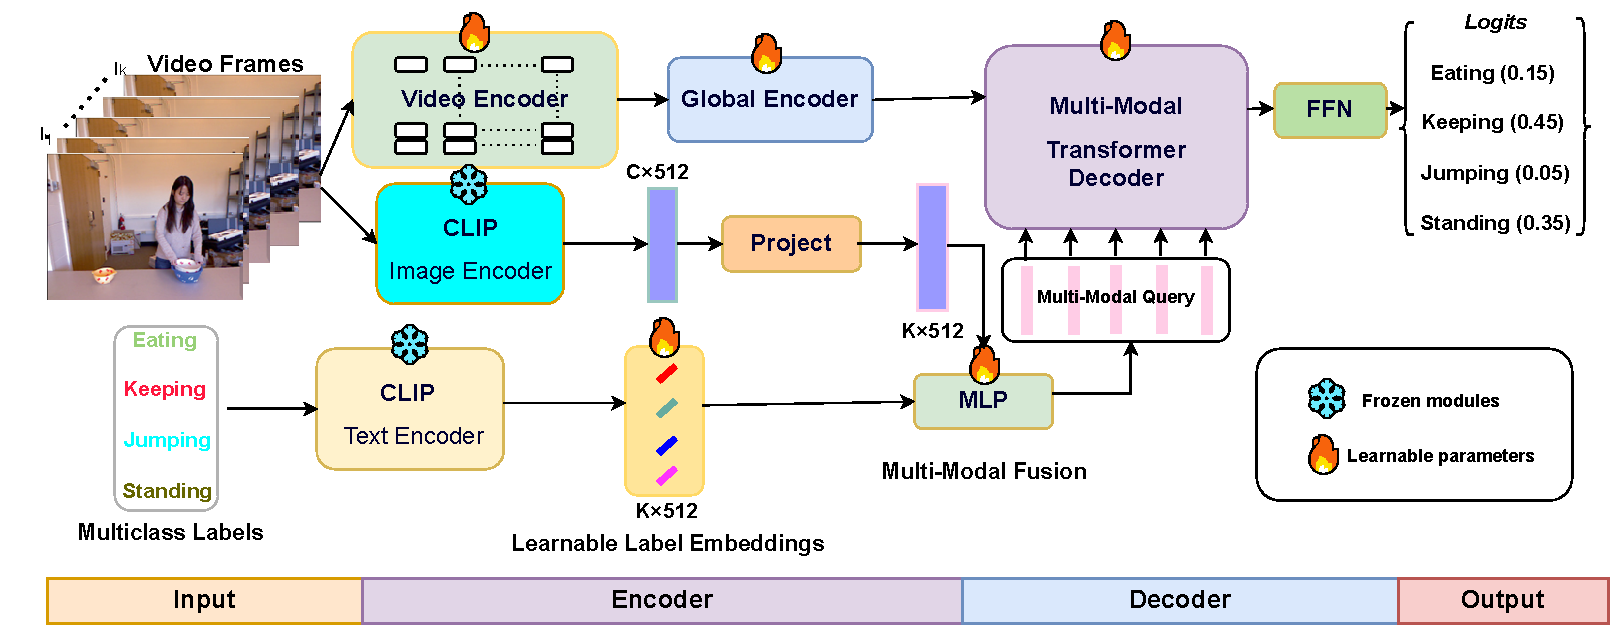
\includegraphics[width=1.0\textwidth]{assets/charts_rw/MSQNet}
    \caption[Model Structure of MSQNet]{Illustration of MSQNet's model structure. Source \parencite{mondal2023msqnet}}
    \label{fig:discussion_msqnet}
\end{figure}

Figure \ref{fig:discussion_msqnet} presents the model structure of MSQNet. The core module of this structure is the Multi-Modal Transformer Decoder (MMTD). The entire structure can be divided into three parts: 

\begin{enumerate}
    \item \textbf{Key and Value of MMTD}: The input video $X \in \mathbf{R}^{N, T, C, H, W}$ is processed by the video encoder, specifically the TimeSformer, where $N$ represents the batch size, $T$ represents the number of frames, and C, H and W represents the channels, width and height of a frame, respectively. By averaging pooling patch embeddings generated by the video encoder within the same frame, frame-level embeddings are obtained. These embeddings are subsequently multiplied by the projection weights $W \in \mathbf{R}^{D \times D}$ to yield the key and value of the MMTD in the shape $(N, D)$. 
    \item \textbf{Query of MMTD}: The video embedding $Q_v \in \mathbf{R}^{N \times D}$ is derived from the average pooling of frame embeddings encoded by the image encoder of CLIP. The learnable class embedding $Q_l \in \mathbf{R}^{K \times D}$ is initialised with the text encoder of CLIP, taking the original label text as input, where $K$ denotes the number of classes. To produce a query $Q \in \mathbf{R}^{K \times D}$, the embeddings $Q_v$ and $Q_l$ are concatenated, resulting in $Q \in \mathbf{R}^{K \times 2D}$, which is then projected using the weight $W \in \mathbf{R}^{2D \times D}$. 
    \item \textbf{operation of MMTD}: Several layers of the cross-attention mechanism are applied to the query, key, and value to produce the embedding for each class $Q^l \in \mathbf{R}^{K \times D}$, where $l \in L$ represents the. This is then followed by an FFN module to produce the class logits.
\end{enumerate}

\subsection{Comparison}
Three key differences exist between AFRICAN and MSQNet: 

\begin{enumerate}
    \item \textbf{Cross-Attention}: The cross-attention mechanism enables the model to compute attention between the label embeddings and frame-level embedding, which is the most meticulously designed mechanism in this structure.
    \item \textbf{Learnable label Embedding}: Unlike AFRICAN, which uses fixed label embedding, MSQNet initialises the learnable label embedding with values produced by the pretrained CLIP model. This allows the model to update the weights of the label embedding to fit better.
    \item \textbf{Fusion of Image and Text Embedding}: Instead of adopting CLIP's similarity calculation method, MSQNet concatenates the text and video embeddings with a projection layer to fuse them together. 
\end{enumerate}

These features make MSQNet more adaptable to fit on a medium-sized dataset. On the contrary, AFRICAN tries to mimic the training scheme to directly calculate the image-text similarity for action recognition. Although this enables the model to update a minimum number of parameters to achieve an acceptable result, it restricts the model's potential to better fit the data. Given that MSQNet was published a month prior to the submission of this dissertation and their code is not yet publicly available, the improvement may be further studied in the future.

\subsection{Implementation}
To better quantify the improvement caused by the three differences mentioned above. I do the following three experiments

\begin{enumerate}
    \item \textbf{}: 
    \item \textbf{}
    \item \textbf{}
    \item \textbf{}
\end{enumerate}




learnable label embedding
LLE
\begin{table}[ht]
    \centering
    \caption[] {}
    \label{tab:ablation_vc}
    \begin{tabular}{lllll}
        \toprule
        \multirow{2}{*}{Models} & Accuracy \\
        \cmidrule{2-2} 
        {} &  Best Epoch \\
        \midrule
        VC\_DF & 25.74 \\
        MSQ_TS_LLE   & 48.56 \\
        MSQ_VC_LLE   & 48.56 \\
        MSQ_TS_LLE         & 54.36 \\
        VC\_AT     & 52.79 \\
        VC\_DF     & 55.98 \\
        \bottomrule
    \end{tabular}
\end{table}



Test Test Test Test Test Test Test Test Test Test Test Test Test Test Test Test Test Test Test Test Test Test Test Test Test Test Test Test Test Test Test Test Test Test Test Test Test Test Test Test Test Test Test Test Test Test Test Test Test Test Test Test Test Test Test Test Test Test Test Test Test Test Test Test.
Test Test Test Test Test Test Test Test Test Test Test Test Test Test Test Test Test Test Test Test Test Test Test Test Test Test Test Test Test Test Test Test Test Test Test Test Test Test Test Test Test Test Test Test Test Test Test Test Test Test Test Test Test Test Test Test Test Test Test Test Test Test Test Test.
Test Test Test Test Test Test Test Test Test Test Test Test Test Test Test Test Test Test Test Test Test Test Test Test Test Test Test Test Test Test Test Test Test Test Test Test Test Test Test Test Test Test Test Test Test Test Test Test Test Test Test Test Test Test Test Test Test Test Test Test Test Test Test Test.
Test Test Test Test Test Test Test Test Test Test Test Test Test Test Test Test Test Test Test Test Test Test Test Test Test Test Test Test Test Test Test Test Test Test Test Test Test Test Test Test Test Test Test Test Test Test Test Test Test Test Test Test Test Test Test Test Test Test Test Test Test Test Test Test.
Test Test Test Test Test Test Test Test Test Test Test Test Test Test Test Test Test Test Test Test Test Test Test Test Test Test Test Test Test Test Test Test Test Test Test Test Test Test Test Test Test Test Test Test Test Test Test Test Test Test Test Test Test Test Test Test Test Test Test Test Test Test Test Test.
Test Test Test Test Test Test Test Test Test Test Test Test Test Test Test Test Test Test Test Test Test Test Test Test Test Test Test Test Test Test Test Test Test Test Test Test Test Test Test Test Test Test Test Test Test Test Test Test Test Test Test Test Test Test Test Test Test Test Test Test Test Test Test Test.
% \subsection{The effect smaller of batch size}
% Owing to the 80 Gb limitation of A100 GPU, I am able to train the fully learnable model, VC\_Vision, with a batch size of 16. To investigate the effect of this, I compare the 


% 0.514509499	0.543613255	0.559846222	0.257423162	0.481209993
% VC_AT	    IC	        VC_dd	    VC2_Vision	VC2_Proj
